\definecolor{lightgray}{HTML}{dddddd}
\definecolor{medgray}{HTML}{cccccc}
\definecolor{medgray2}{HTML}{bbbbbb}
\definecolor{darkgray}{HTML}{aaaaaa}
\definecolor{lightgp}{HTML}{ddddee}
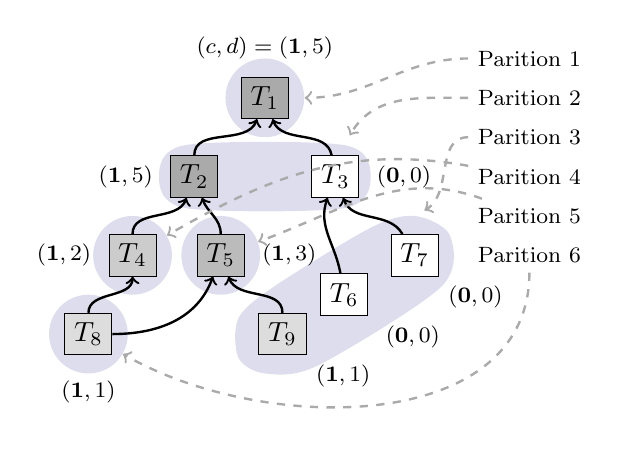
\begin{tikzpicture}[x=1.12cm]
    \begin{scope}[all/.style={draw, minimum height=0.5cm, minimum width=0.5cm},line width=0.08ex]
        \node[fill=lightgp, circle,minimum width=1cm] (pt1) at (0, 0) {};
        \node[fill=lightgp, circle,minimum width=1cm] (pt4) at (-1.5, -2) {};
        \node[fill=lightgp, circle,minimum width=1cm] (pt5) at (-0.5, -2) {};
        \node[fill=lightgp, circle,minimum width=1cm] (pt6) at (-2, -3) {};
        \fill[color=lightgp] plot[smooth cycle] coordinates { (1.2, -1) (0.9, -1.4) (-0.9, -1.4) (-1.2, -1) (-0.9, -0.6) (0.9, -0.6)} node (pt2) {};
        \fill[color=lightgp] plot[smooth cycle] coordinates {(2.1, -1.75) (2, -2.4) (0.6, -3.4) (0, -3.5) (-0.3, -3.3)(-0.3, -2.8) (0.1, -2.4) (1.2, -1.65) (1.7, -1.5) } node (pt3) {};
        \node[all, draw,fill=darkgray] (b0) at (0, 0) {$T_1$};
        \node[all, draw,fill=darkgray] (b1) at (-0.8, -1) {$T_2$};
        \node[all, draw,fill=white] (b2) at (0.8, -1) {$T_3$};
        \node[all, draw,fill=medgray] (b3) at (-1.5, -2) {$T_4$};
        \node[all, draw,fill=medgray2] (b4) at (-0.5, -2) {$T_5$};
        \node[all, draw,fill=white] (b5) at (0.9, -2.5) {$T_6$};
        \node[all, draw,fill=white] (b6) at (1.7, -2) {$T_7$};
        \node[all, draw,fill=lightgray] (b7) at (-2, -3) {$T_8$};
        \node[all, draw,fill=lightgray] (b8) at (0.2, -3) {$T_9$};
        \begin{scope}[line width=0.2ex]
        \path[->] (b1) edge[out=90, in=-110] node[sloped,above] {} (b0) ;
        \path[->] (b2) edge[out=100, in=-70] node[sloped,above] {} (b0) ;
        \path[->] (b3) edge[out=90, in=-110] node[sloped,above] {} (b1) ;
        \path[->] (b4) edge[out=90, in=-70] node[sloped,above] {} (b1) ;
        \path[->] (b5) edge[out=100, in=-110] node[sloped,above] {} (b2) ;
        \path[->] (b6) edge[out=120, in=-70] node[sloped,above] {} (b2) ;
        \path[->] (b7) edge[out=90, in=-90] node[sloped,above] {} (b3) ;
        \path[->] (b7) edge[out=0, in=-110] node[sloped,above] {} (b4) ;
        \path[->] (b8) edge[out=90, in=-70] node[sloped,above] {} (b4) ;
        \end{scope}
        \node[anchor=south, yshift=0.1cm] at (b0.north) {\footnotesize$(c, d) = (\textbf{1}, 5)$};
        \node[anchor=east,xshift=-0.1cm] at (b1.west) {\footnotesize$(\textbf{1}, 5)$};
        \node[anchor=west,xshift=0.1cm] at (b2.east) {\footnotesize$(\textbf{0}, 0)$};
        \node[anchor=east,xshift=-0.1cm] at (b3.west) {\footnotesize$(\textbf{1}, 2)$};
        \node[anchor=west,xshift=0.1cm] at (b4.east) {\footnotesize$(\textbf{1}, 3)$};
        \node[anchor=north west,xshift=0.1cm] at (b5.south east) {\footnotesize$(\textbf{0}, 0)$};
        \node[anchor=north west] at (b6.south east) {\footnotesize$(\textbf{0}, 0)$};
        \node[anchor=north west] at (b8.south east) {\footnotesize$(\textbf{1}, 1)$};
        \node[anchor=north,yshift=-0.2cm] at (b7.south) {\footnotesize$(\textbf{1}, 1)$};
        \node[] (p1) at (3, 0.5) {\footnotesize$\textrm{Parition 1}$};
        \node[] (p2) at (3, 0) {\footnotesize$\textrm{Parition 2}$};
        \node[] (p3) at (3, -0.5) {\footnotesize$\textrm{Parition 3}$};
        \node[] (p4) at (3, -1) {\footnotesize$\textrm{Parition 4}$};
        \node[] (p5) at (3, -1.5) {\footnotesize$\textrm{Parition 5}$};
        \node[] (p6) at (3, -2) {\footnotesize$\textrm{Parition 6}$};
        \begin{scope}[color=darkgray,dashed,line width=0.2ex]
        \path[->] (p1) edge[out=180, in=0] node[sloped,above] {} (pt1) ;
        \path[->] (p2) edge[out=180, in=60] node[sloped,above] {} (pt2) ;
        \path[->] (p3) edge[out=180, in=30] node[sloped,above] {} (pt3) ;
        \path[->] (p4) edge[out=170, in=30] node[sloped,above] {} (pt4) ;
        \path[->] (p5) edge[out=160, in=20] node[sloped,above] {} (pt5) ;
        \path[->] (p6) edge[out=270, in=-30] node[sloped,above] {} (pt6) ;
        \end{scope}
    \end{scope}
\end{tikzpicture}
